\documentclass[12pt,a4paper]{report}  

\usepackage{graphicx}
\usepackage{longtable}
\usepackage{float}
\usepackage{fancyhdr}
\usepackage{titlesec}
\usepackage{helvet}
\renewcommand{\familydefault}{\sfdefault}
\usepackage{listings}
\usepackage{xcolor}
\usepackage{lipsum}
\usepackage{geometry} 
\usepackage{setspace}
\usepackage[backend=biber,style=numeric]{biblatex}
\usepackage{tikz}
\usetikzlibrary{fadings}
\geometry{margin=1in}

\addbibresource{references.bib}

\setcounter{secnumdepth}{4}
\setcounter{tocdepth}{4}

% Code Style
\lstdefinestyle{csharpstyle}{
  language=PHP,
  basicstyle=\ttfamily\small,
  keywordstyle=\color{blue},
  commentstyle=\color{gray},
  stringstyle=\color{red},
  tabsize=4,
  showspaces=false,
  showstringspaces=false,
  breaklines=true,
  numbers=none
}

% Chapter Formatting
\titleformat{\chapter}
  {\vspace{-2cm} \centering\bfseries\LARGE}
  {\thechapter}{1em}{}  

\begin{document}

\begin{titlepage}
    % Background Image & Gradient overlay matching the HTML CSS specs
    \begin{tikzpicture}[remember picture, overlay]
        % The bottom image container (42% height)
        \node[anchor=south, inner sep=0, outer sep=0] at (current page.south) {
            \includegraphics[width=\paperwidth, height=0.42\paperheight]{logo.png}
        };
        % The linear gradient overlay (fading from white to transparent over 65% of the 42% container)
        % 0.42 * 0.65 = 0.273. It fades from 0.42 down to 0.42 - 0.273 = 0.147
        \fill[white, path fading=south] 
            ([yshift=0.42\paperheight]current page.south west) rectangle ([yshift=0.147\paperheight]current page.south east);
        % Tiny buffer to ensure no harsh line at the exact top pixel of the image
        \fill[white] ([yshift=0.419\paperheight]current page.south west) rectangle ([yshift=0.43\paperheight]current page.south east);
    \end{tikzpicture}

    \vspace*{0.5cm}
    \begin{center}
        {\fontsize{17pt}{22pt}\selectfont\textbf{DEPARTMENT OF COMPUTER SCIENCE\\[0.1cm]RAJAGIRI COLLEGE OF SOCIAL SCIENCES\\[0.1cm](AUTONOMOUS)\\[0.1cm]KALAMASSERY-KOCHI-683104}}\\[1.2cm]
        
        
\includegraphics[height=3.5cm]{RCSS.png}\\[1.2cm]
        
        {\fontsize{16pt}{20pt}\selectfont\textbf{BSc Computer Science (Hons.) Data Analytics}}\\[0.4cm]
        {\fontsize{15pt}{20pt}\selectfont\textbf{WPL Project Report}}\\[0.8cm]
        
        {\fontsize{34pt}{40pt}\selectfont\textbf{Top Score}}\\[0.2cm]
        {\fontsize{19pt}{24pt}\selectfont\textbf{Quiz System}}\\[1.2cm]
        
        \begin{tabular}{l c l}
            \textbf{\fontsize{14pt}{20pt}\selectfont Name} & \textbf{\fontsize{14pt}{20pt}\selectfont :} & \textbf{\fontsize{14pt}{20pt}\selectfont Nakul Sreekumar} \\[0.2cm]
            \textbf{\fontsize{14pt}{20pt}\selectfont Semester} & \textbf{\fontsize{14pt}{20pt}\selectfont :} & \textbf{\fontsize{14pt}{20pt}\selectfont 4th Semester} \\[0.2cm]
            \textbf{\fontsize{14pt}{20pt}\selectfont Register No.} & \textbf{\fontsize{14pt}{20pt}\selectfont :} & \textbf{\fontsize{14pt}{20pt}\selectfont 24118018} \\
        \end{tabular}
    \end{center}
    
    \vfill
\end{titlepage}

\newpage
\include{certificate}
\newpage

\setstretch{1.15}

\pagenumbering{roman}
\include{acknowledgement}
\newpage
\chapter*{ \begin{center} 
    \textbf{\LARGE ABSTRACT}  % Large, bold, and centered heading  
\end{center} }  
\addcontentsline{toc}{chapter}{ABSTRACT}  
\vspace{-2cm}  % Adjust this value if needed to reduce space further  
 

 The Top Score Quiz System is a comprehensive web-based application developed to automate and manage online assessments and quizzes efficiently. The system provides a centralized platform for educational institutions and organizations to create, manage, and evaluate quizzes seamlessly without the overhead of traditional paper-based methods. It replaces manual evaluation processes with an automated grading system, thereby improving operational efficiency, reducing human errors, and enhancing the overall learning experience.
\\\\
The application implements role-based access control to ensure secure interaction among users such as Admin, Teacher, and Student. The Admin module oversees user management and system integrity. Teachers can create dynamic quizzes, add multiple-choice or true/false questions, and monitor student performance in real-time. Students can join quizzes using a unique access code, participate in timed assessments, and view their immediate results and detailed reviews upon completion.
\\\\
A key feature of the system allows teachers to bulk upload questions using CSV formats and share quiz access codes easily. Developed using the Laravel framework with a MySQL database, the system ensures data security, scalability, and high performance. By centralizing the assessment workflow and digitizing academic evaluations, the Top Score Quiz System significantly improves administrative efficiency and supports modern educational practices.\\\\

\newpage



% List of Tables
\addcontentsline{toc}{chapter}{LIST OF TABLES}
\renewcommand{\listtablename}{\hfill \LARGE \textbf{LIST OF TABLES} \hfill}
\listoftables
\newpage

% List of Figures
\addcontentsline{toc}{chapter}{LIST OF FIGURES}
\renewcommand{\listfigurename}{\hfill \LARGE \textbf{LIST OF FIGURES} \hfill}
\listoffigures
\newpage

% Table of Contents
\renewcommand{\contentsname}{\hfill \LARGE \textbf{CONTENTS} \hfill}
\tableofcontents
\newpage

% ===============================
% HEADER & FOOTER SETTINGS
% ===============================

\pagestyle{fancy}
\fancyhf{}

\fancyhead[R]{Top Score Quiz System}

\renewcommand{\footrulewidth}{0.4pt}
\fancyfoot[L]{Department of Computer Science, RCSS}
\fancyfoot[R]{\thepage}

% Plain pages (chapter first pages)
\fancypagestyle{plain}{
    \fancyhf{}
    \fancyhead[R]{Top Score Quiz System}
    \renewcommand{\footrulewidth}{0.4pt}
    \fancyfoot[L]{Department of Computer Science, RCSS}
    \fancyfoot[R]{\thepage}
}

% Page style without header/footer if needed
\fancypagestyle{noheaderfooter}{
    \fancyhf{}
    \renewcommand{\headrulewidth}{0pt}
    \renewcommand{\footrulewidth}{0pt}
}

\pagenumbering{arabic}

% ===============================
% MAIN CONTENT
% ===============================

\chapter{INTRODUCTION}

In today’s educational and corporate environments, efficient management of assessments, quizzes, and performance tracking is essential for evaluating knowledge effectively. Traditional examination systems that rely heavily on manual test paper generation, physical distribution, and manual grading often result in a slow turnaround time, increased human error, and difficulties in maintaining historical performance records. To overcome these limitations, institutions require an integrated and automated digital assessment solution.

The Top Score Quiz System is a web-based application developed to streamline and automate the entire quiz lifecycle through a centralized and secure platform. The system integrates multiple user personas—including Administrators, Teachers, and Students—into a unified digital ecosystem. It ensures smooth execution of assessments, reduces manual grading workload, and enhances evaluation transparency.

The system implements role-based access control, allowing different users to perform tasks according to their responsibilities:
\begin{itemize}
    \item \textbf{Administrators:} Manage platform users, oversee system operations, and ensure a secure environment.
    \item \textbf{Teachers:} Manage quizzes, add diverse question types (Multiple Choice, True/False) manually or via CSV uploads, set time limits, share unique access codes, and analyze overall student performance.
    \item \textbf{Students:} Register securely, join active quizzes using specialized access codes, complete timed assessments, and review their scores and correct answers immediately after submission.
\end{itemize}

In addition to traditional quiz generation, the system provides flexibility by allowing teachers to review detailed student attempts, including identifying areas where students frequently make mistakes. Students benefit from an intuitive interface that tracks their time remaining during a quiz and displays comprehensive results.

Developed using the Laravel framework and MySQL database, the Top Score Quiz System ensures data security, scalability, and performance efficiency. By digitizing assessments and automating grading workflows, the system enhances administrative control, improves the quality of feedback for learners, and supports modern e-learning delivery.

\section{Supporting Literature}

The evolution of modern e-learning platforms highlights a significant transition from paper-based assessment methodologies to digital execution environments. Recent academic studies underscore that digital assessment systems dramatically reduce evaluator bias while enabling instantaneous, data-driven feedback architectures—a critical component for iterative learning. Furthermore, robust web frameworks like Laravel enforce the Model-View-Controller (MVC) architectural pattern, which academic and industry literature agrees is essential for decoupling backend business logic from user interface presentation. This ensures a maintainable repository that can adapt to changing educational requirements rapidly.

Role-based access controls (RBAC), as implemented in the Top Score Quiz System, are also cited as foundational elements in Learning Management Systems (LMS). By completely partitioning Administrator, Teacher, and Student scopes, platform data integrity is highly fortified against unauthorized modifications.

\section{Report Structure}

This report extensively documents the fundamental design paradigms underpinning the Top Score Quiz System. To thoroughly contextualize the application's architecture, Chapter 4 encompasses the \textbf{System Design}, which exclusively features the \textbf{Class Diagram}—illustrating the programmatic objects, their attributes, and interdependent methods—as well as the detailed \textbf{Entity-Relationship (ER) Diagram}, which meticulously maps the underlying MySQL relational schema that supports the system logic.

\chapter{SYSTEM ANALYSIS}

\section{Module Description}

The Top Score Quiz System is divided into multiple functional modules, each responsible for managing specific assessment and evaluation operations efficiently. The major modules are described below:

\begin{itemize}

\item \textbf{User Management Module:}
This module manages registration, authentication, and role-based access control for all users including Admins, Teachers, and Students. It ensures secure login and restricts access to system features based on the designated user roles.

\item \textbf{Quiz Creation and Management Module:}
This module empowers Teachers to create, edit, and manage quizzes. It involves defining quiz titles, time limits (duration), passing criteria, and generating unique access codes used by students to join the specific quiz session.

\item \textbf{Question Bank Module:}
This module enables Teachers to construct the content of the quizzes. It supports adding diverse question formats such as Multiple Choice Questions (MCQs) and True/False parameters. It also supports bulk question imports via CSV files for rapid assessment generation.

\item \textbf{Assessment Execution Module:}
This module allows Students to enter a unique quiz code, join the session, and take the timed test. Built-in timers ensure adherence to the test duration constraints, and progress is tracked throughout the quiz taking process.

\item \textbf{Grading and Results Module:}
This module automates the evaluation of student submissions. It calculates scores instantly based on predefined correct answers and records the attempt details in the database. Students can review their individual performance, while Teachers can access consolidated performance statistics across all participants.

\end{itemize}

\section{Business Rules}

Business rules define operational constraints to ensure system consistency and reliability.

\textbf{User and Access Rules}
\begin{itemize}
\item Every user must register and authenticate before accessing the system.
\item Role-based access control restricts access; for example, Students cannot modify quizzes.
\item Only Administrators have the authority to manage overarching system users.
\end{itemize}

\textbf{Quiz and Assessment Rules}
\begin{itemize}
\item A quiz cannot be accessed by a student without the exact unique access code.
\item Once a time limit expires during an active quiz attempt, the system must automatically submit the current progress.
\item A student’s final score is calculated immediately upon submission.
\end{itemize}

\textbf{Question Management Rules}
\begin{itemize}
\item Only the Teacher who created the quiz can add or modify its questions.
\item Each question must explicitly define a correct answer during creation to enable automated grading.
\item Uploaded CSV files for question imports must follow the predefined structured template.
\end{itemize}


\section{Analysis of Architecture}

The Top Score Quiz System follows the Laravel MVC (Model–View–Controller) architecture to ensure structured and maintainable development.

\begin{enumerate}

\item \textbf{Model Layer:}
Handles database interactions using the Eloquent ORM. It defines relationships between entities such as User, Quiz, Question, Result, and StudentAnswers. For instance, a Quiz has many Questions, and a User has many Results.

\item \textbf{View Layer:}
Developed using the Blade templating engine (accompanied by HTML, CSS, and JavaScript) to display role-specific dashboards, interactive quiz-taking interfaces, and dynamic result data.

\item \textbf{Controller Layer:}
Manages request handling, validation, business logic processing (like timer validation and score calculation), and user redirection (e.g., `QuizController`).

\item \textbf{Database Layer:}
Uses MySQL for storing structured academic data including users, quizzes, corresponding questions, and recorded student attempts securely.

\item \textbf{Security Features:}
Implements password hashing, CSRF protection, middleware-based role gating (`role:admin`, `role:teacher`, `role:student`), and database transaction protections for data safety.

\end{enumerate}

\section{Feasibility Analysis}

\subsection{Technical Feasibility}

The system is developed using the robust Laravel framework and MySQL database, which are reliable, scalable, and extensively supported technologies. The application can run on standard web servers (Apache or Nginx) and can be deployed easily in an institutional environment. The standardized development approach guarantees maintainability and future expandability.

\subsection{Economic Feasibility}

The project is highly cost-effective as it heavily utilizes open-source technologies (PHP, Laravel, MySQL). Development and maintenance costs are relatively minimal. The automated grading features significantly reduce manual paperwork and staffing overhead associated with test evaluations.

\subsection{Operational Feasibility}

The system interface is designed to be highly intuitive, aligning with typical e-learning paradigms. Teachers and Students can effortlessly adopt the digital system without extensive training. The compartmentalized modules ensure smooth daily academic operations and swift quiz deployments.

\section{System Environment}

\subsection{Software Environment}

\textbf{Operating System:} Windows 10/11, macOS, or Linux \\
\textbf{Backend Framework:} Laravel 11.x \\
\textbf{Programming Language:} PHP 8.2+ \\
\textbf{Frontend:} Blade Templates, HTML5, CSS3, JavaScript \\
\textbf{Database:} MySQL 8.0+ \\
\textbf{Web Server:} Apache / Nginx \\
\textbf{Development Tools:} VS Code, Composer, Git \\

\subsection{Hardware Environment}

\textbf{Processor:} Intel Core i3 / AMD Ryzen 3 or higher \\
\textbf{Memory (RAM):} 8 GB minimum (16 GB optimal for development) \\
\textbf{Storage:} 256 GB SSD \\
\textbf{Operating System:} Windows 11 \\

\section{Actors and Roles}

\textbf{Administrator}
\begin{itemize}
\item Manage and monitor registered users across the platform.
\item Oversee application stability and manage global settings.
\item Handle potential user account deletions and moderation.
\end{itemize}

\textbf{Teacher}
\begin{itemize}
\item Construct new quizzes with customizable settings (duration, titles).
\item Populate quizzes with questions manually or via CSV imports.
\item Distribute unique quiz access codes to target students.
\item Monitor ongoing assessments and review comprehensive student results.
\end{itemize}

\textbf{Student}
\begin{itemize}
\item Register and securely sign into the learning platform.
\item Join specific quizzes using unique access codes provided by Teachers.
\item Attempt quizzes within the allocated timeframe and submit answers.
\item View detailed post-quiz performance reports and correct answer keys.
\end{itemize}

\chapter{SYSTEM DESIGN }

 \section{Use case model}
\begin{figure}[H]
    \centering
    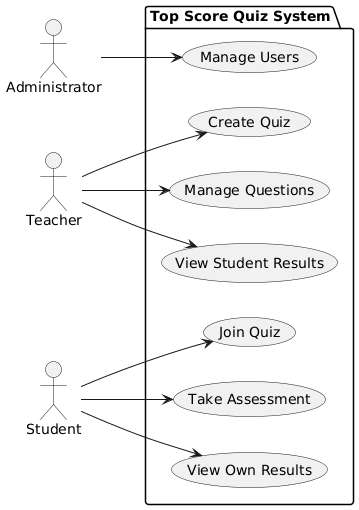
\includegraphics[width=1\textwidth,height=0.9\textwidth]{UseCase_Diagram.png}
    \caption{Use case Diagram}
    \label{fig:Use_case}
\end{figure}
This Use Case Diagram illustrates the interactions between users and the Top Score Quiz System. The Administrator manages overarching users and platform stability. The Teacher creates quizzes, adds questions, defines settings, manages quiz access codes, and reviews student results. The Student registers, joins particular quizzes using an access code, answers questions within a time constraint, submits their responses, and views instantaneous feedback.

 \section{Activity Diagram}
 \subsection{Teacher Creating Quiz}
\begin{figure}[H]
    \centering
    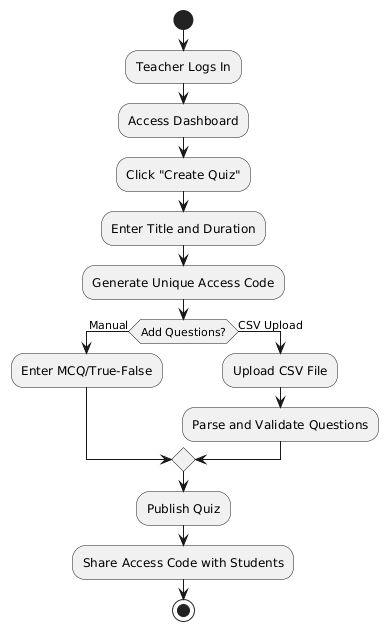
\includegraphics[width=1\textwidth,height=0.9\textwidth]{Teacher_Create_Quiz_Activity.png}
    \caption{Teacher Creating Quiz Activity diagram}
    \label{fig:Activity_1}
\end{figure}
This Activity Diagram represents the Quiz Creation process in the Top Score Quiz System. The process begins when a Teacher logs into the system and accesses the Teacher Dashboard. The Teacher selects "Create Quiz" and inputs details such as the title and duration. Upon hitting submit, a unique access code is generated automatically. Following this, the Teacher builds the quiz by manually adding questions (MCQ or True/False) or uploading a formatted CSV file. Finally, the quiz is published and the access code is shared with students.

\subsection{Student Taking Quiz}
\begin{figure}[H]
    \centering
    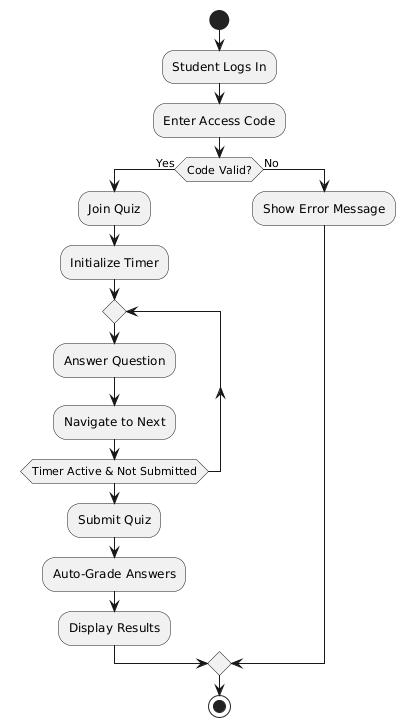
\includegraphics[width=0.5\textwidth]{Student_Take_Quiz_Activity.png}
    \caption{Student Taking Quiz Activity Diagram}
    \label{fig:Activity_2}
\end{figure}
This Activity Diagram represents the process of a Student joining and completing an assessment. The Student navigates to the Student Dashboard and inputs a provided access code. If the code is invalid, they are denied entry. If valid, the quiz environment is initialized and a countdown timer begins. The Student navigates through the questions, interacting with the system to save their responses. Once the timer expires or the Student manually submits the test, the system validates the answers against the database, immediately generates a score, and presents the final evaluation to the Student.

\section{Sequence Diagram}

\subsection{Student Quiz Submission Sequence}

\begin{figure}[H]
    \centering
    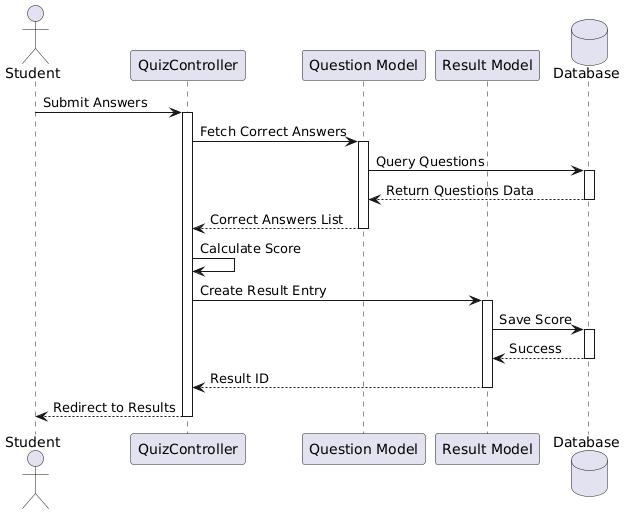
\includegraphics[width=0.9\textwidth]{Quiz_Submission_Sequence.png}
    \caption{Student Quiz Submission Sequence Diagram}
    \label{fig:Sequence_1}
\end{figure}

This sequence diagram illustrates the interaction between the Student, the QuizController, the Question Repository, and the Results Database during a quiz submission. The Student clicks "Submit" (or the timer triggers an auto-submit). The QuizController gathers the array of submitted answers and fetches the accurate 'correct\_answer' values from the Question Repository. It iterates through the student's choices, calculating the accumulated score. Finally, the total score and discrete student\_answers are logged into the Results Database, and a success response and redirect view are sent back to the Student's interface.

\section{Class Diagram}
\begin{figure}[H]
    \centering
    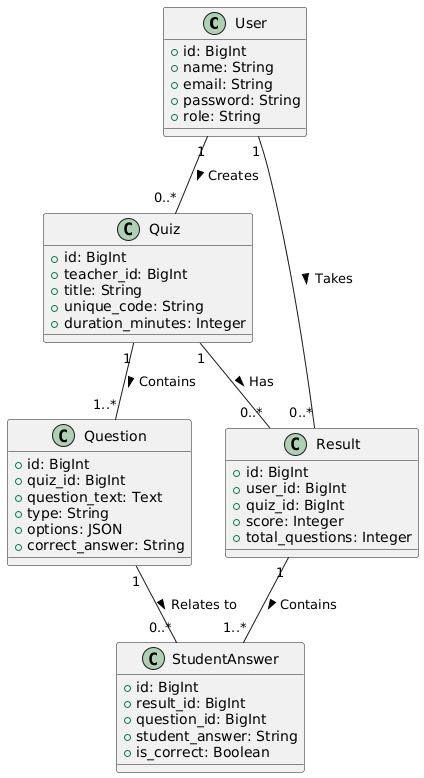
\includegraphics[width=1\textwidth]{Class_Diagram.png}
    \caption{Class Diagram}
    \label{fig:Class_Diagram}
\end{figure}
This Class Diagram represents the static structure of the Top Score Quiz System. It highlights the primary classes—such as User, Quiz, Question, and Result—along with their attributes, methods, and the relationships between them, illustrating how data is encapsulated and manipulated within the system's architecture.

\section{Entity-Relationship (ER) Diagram}
\begin{figure}[H]
    \centering
    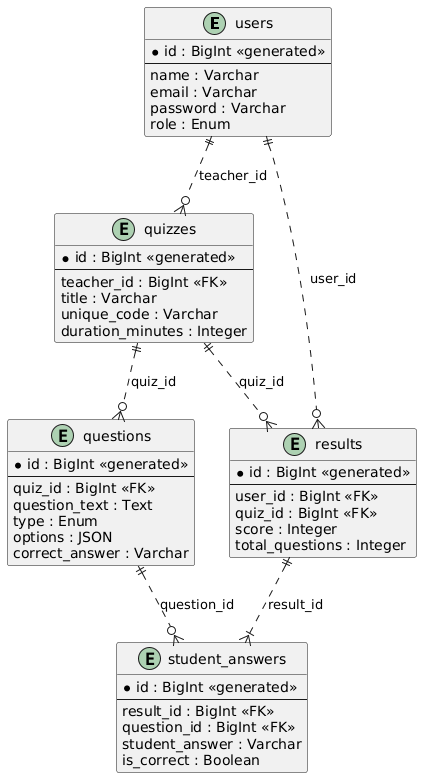
\includegraphics[width=1\textwidth,height=0.8\textwidth]{ER_Diagram.png}
    \caption{Entity-Relationship Diagram}
    \label{fig:ER_Diagram}
\end{figure}
The Entity-Relationship (ER) Diagram models the logical structure of the database. It defines the core entities—Users, Quizzes, Questions, Results, and Student Answers—and the cardinal relationships connecting them. This serves as the foundation for the relational database schema implemented in MySQL.

\section{Project Design}

System design is the process of defining the architecture, components, modules, interfaces, and data flow of a system to meet specified requirements. It ensures that the system is structured, scalable, secure, and user-friendly. Good system design focuses on usability, efficiency, performance, and data security while maintaining clear role-based responsibilities and workflow management. 

In the Top Score Quiz System, the design focuses on ensuring seamless execution of structured tests between Teachers and Students. The system integrates robust session management and data verification to maintain the academic integrity of the quizzes (e.g., verifying a user didn't modify time constraints). The system balances complex underlying evaluations with a streamlined dashboard experience for ease of use.

\subsection{UI Design}

The User Interface (UI) design of Top Score is structured to be distraction-free, modern, and purely functional. Each user type—Admin, Teacher, and Student—has a distinct dashboard displaying relevant tools.

\begin{figure}[H]
    \centering
    \includegraphics[width=1\textwidth]{image_0.png}
    \caption{Landing / Login Interface}
    \label{fig:Screenshot_1}
\end{figure}

The UI includes:
\begin{itemize}
    \item A streamlined Student interface emphasizing active quizzes, a prominent join-code input, and clear visual timers during assessments.
    \item A comprehensive Teacher dashboard displaying a list of their owned quizzes, tools to manage questions, and detailed tabular formats for student result evaluations.
    \item Clean authentication forms and straightforward navigational menus adhering to contemporary frontend standards.
\end{itemize}

\begin{figure}[H]
    \centering
    \includegraphics[width=1\textwidth]{image_1.png}
    \caption{Teacher Dashboard}
    \label{fig:Screenshot_2}
\end{figure}

\begin{figure}[H]
    \centering
    \includegraphics[width=1\textwidth]{image_4.png}
    \caption{Student Dashboard}
    \label{fig:Screenshot_5}
\end{figure}

\subsection{User Interaction Design}

The system is engineered for prompt feedback. Interactions like joining a quiz validate access codes synchronously and throw immediate alerts if incorrect. When a student takes a quiz, the system actively updates them on their remaining time and allows them to navigate questions flexibly before the final submission.

\begin{figure}[H]
    \centering
    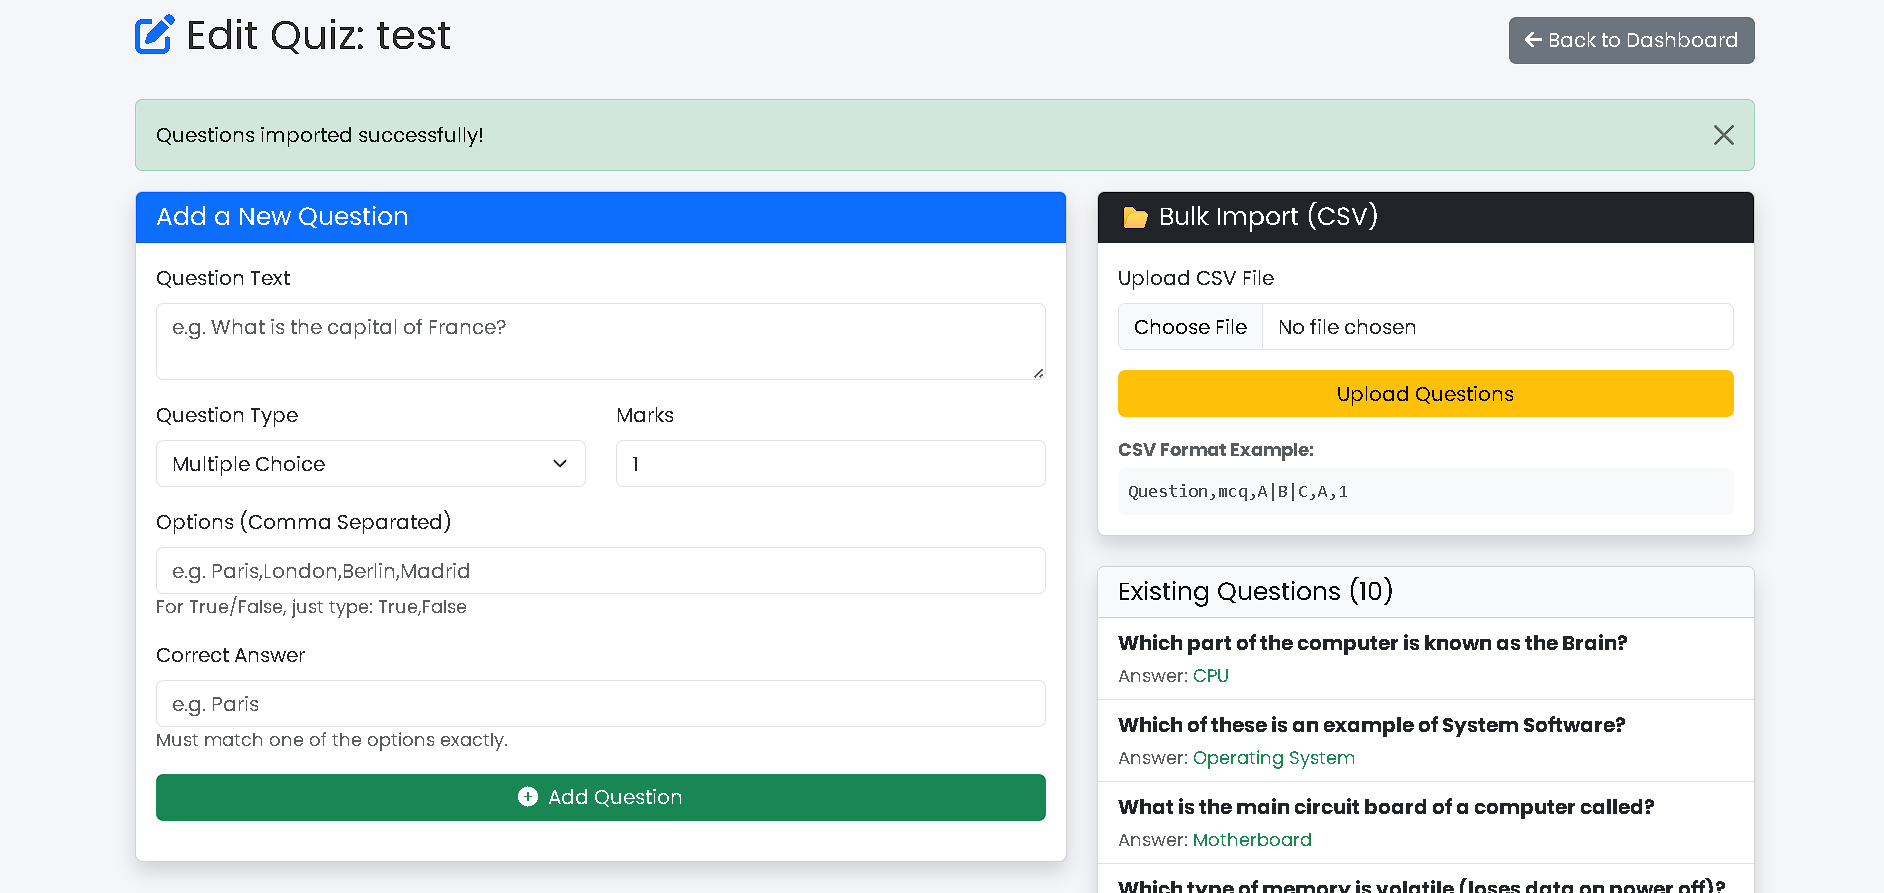
\includegraphics[width=1\textwidth]{quiz creation.png}
    \caption{Teacher Quiz Creation Page}
    \label{fig:Screenshot_3}
\end{figure}

Role-based interaction ensures:
\begin{itemize}
    \item Students are sandboxed within their active attempts and previous results summaries.
    \item Teachers control the pacing and distribution of their instructional material.
    \item Accidental double-submissions are mitigated through prompt UI state changes and controller-level restrictions upon pressing "Submit."
\end{itemize}

\subsection{Grading and Evaluation Design}

The system uses a synchronous grading algorithm executed entirely on the server side to prevent tampering. Every question carries a designated weight/mark (defaulting to 1). Upon submission, the student's payload is evaluated rigorously against the stored correct answers. The resulting metadata, including total points, potential grades (e.g., Pass/Fail threshold), and individual erroneous answers, are stored persistently for identical post-test reviews for both Student and Teacher.

\begin{figure}[H]
    \centering
    \includegraphics[width=1\textwidth]{image_3.png}
    \caption{Teacher - Class Performance Metrics}
    \label{fig:Screenshot_4}
\end{figure}

\subsection{Project Pipeline}
The project pipeline outlines the systematic flow from initial HTTP request to database transaction and back to the client interface. The standard Laravel architecture handles this through the following steps:
\begin{enumerate}
    \item \textbf{Routing:} Incoming HTTP requests are intercepted by \texttt{web.php} and mapped to appropriate Controller methods.
    \item \textbf{Middleware:} Authentication and role-based checks (e.g., verifying Teacher vs. Student roles) are enforced before execution.
    \item \textbf{Controller Logic:} The designated Controller processes the request, validates input data, and triggers necessary business logic.
    \item \textbf{Model \& Database Interaction:} Eloquent ORM Models interact securely with the MySQL database to retrieve or store information dynamically.
    \item \textbf{View Rendering:} The Controller passes formatted data to Blade templates to construct the frontend HTML presentation logically.
\end{enumerate}

\subsection{Database Design}

The database design follows a strict relational structure using MySQL. The system consists of standard framework tables (\texttt{cache}, \texttt{cache\_locks}, \texttt{failed\_jobs}, \texttt{job\_batches}, \texttt{jobs}, \texttt{migrations}, \texttt{password\_reset\_tokens}, \texttt{sessions}) and primary system entities. The core tables are elaborated in the data dictionary below:

\subsubsection{Data Dictionary}

\begin{table}[H]
    \centering
    \begin{tabular}{|l|l|l|}
        \hline
        \textbf{Column Name} & \textbf{Data Type} & \textbf{Description} \\
        \hline
        id & BigInt, Auto Increment & Primary Key \\
        name & Varchar(255) & User's full name \\
        email & Varchar(255) & Unique email address \\
        password & Varchar(255) & Hashed password \\
        role & Enum('admin', 'teacher', 'student') & Role for access control \\
        created\_at & Timestamp & Record creation time \\
        updated\_at & Timestamp & Record modification time \\
        \hline
    \end{tabular}
    \caption{Users Table}
    \label{tab:users}
\end{table}

\begin{table}[H]
    \centering
    \begin{tabular}{|l|l|l|}
        \hline
        \textbf{Column Name} & \textbf{Data Type} & \textbf{Description} \\
        \hline
        id & BigInt, Auto Increment & Primary Key \\
        teacher\_id & BigInt & Foreign Key (Users) \\
        title & Varchar(255) & Title of the quiz \\
        unique\_code & Varchar(10) & Unique code to join quiz \\
        duration\_minutes & Integer & Total time for the quiz \\
        created\_at & Timestamp & Record creation time \\
        updated\_at & Timestamp & Record modification time \\
        \hline
    \end{tabular}
    \caption{Quizzes Table}
    \label{tab:quizzes}
\end{table}

\begin{table}[H]
    \centering
    \begin{tabular}{|l|l|l|}
        \hline
        \textbf{Column Name} & \textbf{Data Type} & \textbf{Description} \\
        \hline
        id & BigInt, Auto Increment & Primary Key \\
        quiz\_id & BigInt & Foreign Key (Quizzes) \\
        question\_text & Text & The actual question \\
        type & Enum('mcq', 'true\_false') & Type of question \\
        options & JSON & JSON array of options \\
        correct\_answer& Varchar(255) & Correct option / answer \\
        created\_at & Timestamp & Record creation time \\
        updated\_at & Timestamp & Record modification time \\
        \hline
    \end{tabular}
    \caption{Questions Table}
    \label{tab:questions}
\end{table}

\begin{table}[H]
    \centering
    \begin{tabular}{|l|l|l|}
        \hline
        \textbf{Column Name} & \textbf{Data Type} & \textbf{Description} \\
        \hline
        id & BigInt, Auto Increment & Primary Key \\
        user\_id & BigInt & Foreign Key (Users) \\
        quiz\_id & BigInt & Foreign Key (Quizzes) \\
        score & Integer & Total score obtained \\
        total\_questions & Integer & Total questions in quiz \\
        created\_at & Timestamp & Record creation time \\
        updated\_at & Timestamp & Record modification time \\
        \hline
    \end{tabular}
    \caption{Results Table}
    \label{tab:results}
\end{table}

\begin{table}[H]
    \centering
    \begin{tabular}{|l|l|l|}
        \hline
        \textbf{Column Name} & \textbf{Data Type} & \textbf{Description} \\
        \hline
        id & BigInt, Auto Increment & Primary Key \\
        result\_id & BigInt & Foreign Key (Results) \\
        question\_id & BigInt & Foreign Key (Questions) \\
        student\_answer& Varchar(255) & The option selected \\
        is\_correct & Boolean & If answer was correct \\
        created\_at & Timestamp & Record creation time \\
        updated\_at & Timestamp & Record modification time \\
        \hline
    \end{tabular}
    \caption{Student Answers Table}
    \label{tab:student_answers}
\end{table}

Each entity relies heavily on cascading foreign-key relationships to ensure data consistency (e.g., removing a Quiz automatically flushes associated Questions and local Results). 

\subsection{Workflow Design}

The structural workflow guarantees an intuitive instructional process:

\begin{itemize}
    \item A Teacher logs in, creates a quiz, and receives the auto-generated join code.
    \item The Teacher inserts questions into the Quiz manually or via bulk CSV mechanisms.
    \item The Teacher distributes the access code independently to the target class.
    \item A Student inputs the unique code on their dashboard to enroll.
    \item The Student undertakes the test under a strict timer constraint.
    \item Upon conclusion, the system executes an automated grading protocol and saves the result.
    \item The Student views an immediate personal review, while the Teacher views an aggregated classroom report.
\end{itemize}



\chapter{SYSTEM TESTING}

Testing is a critical phase in the software development lifecycle used to identify errors, ensure all modules work as expected, and guarantee that the final product meets specified requirements. The Top Score Quiz System underwent rigorous testing to validate role-based access, data security, and evaluation accuracy.

\section{Unit Testing}
Unit testing involves verifying individual components or functions of the application independently. For the Quiz System, unit tests focused on individual controller methods:

\begin{table}[H]
    \centering
    \begin{tabular}{|p{4cm}|p{7cm}|l|}
        \hline
        \textbf{Test Module} & \textbf{Description \& Expected Result} & \textbf{Status} \\
        \hline
        Question Import Logic & Verify CSV parsing functions handle valid rows correctly and discard malformed rows without crashing. & Pass \\
        \hline
        Grading Algorithm & Provide mock submissions with intentional errors and verify calculated score matches expected outcome. & Pass \\
        \hline
        Timer Enforcement & Test backend timestamp validation ensuring users cannot intercept the clock to maliciously extend time. & Pass \\
        \hline
    \end{tabular}
    \caption{Unit Testing Cases}
    \label{tab:unit_testing}
\end{table}

\section{Integration Testing}
Integration testing evaluates how different modules perform when combined.

\begin{table}[H]
    \centering
    \begin{tabular}{|p{4cm}|p{7cm}|l|}
        \hline
        \textbf{Test Module} & \textbf{Description \& Expected Result} & \textbf{Status} \\
        \hline
        Quiz-to-Questions & Creating a Question accurately binds to the target Quiz ID and displays instantly for enrolled users. & Pass \\
        \hline
        Submission Mapping & Simulate student payload submission ensuring cascade from \textit{Student Answers} array to final \textit{Result} works. & Pass \\
        \hline
    \end{tabular}
    \caption{Integration Testing Cases}
    \label{tab:integration_testing}
\end{table}

\section{System Testing}
System testing is executed on the completely integrated application to evaluate its end-to-end functionality.

\begin{table}[H]
    \centering
    \begin{tabular}{|p{4cm}|p{7cm}|l|}
        \hline
        \textbf{Test Module} & \textbf{Description \& Expected Result} & \textbf{Status} \\
        \hline
        End-to-End Workflow & Teacher registers, creates quiz, code generated. Student registers, joins quiz, takes test, submits. & Pass \\
        \hline
    \end{tabular}
    \caption{System Testing Cases}
    \label{tab:system_testing}
\end{table}

\section{User Acceptance Testing (UAT)}
UAT ensures that the software can handle real-world tasks and meets user expectations. In the context of Top Score:

\begin{table}[H]
    \centering
    \begin{tabular}{|p{4cm}|p{7cm}|l|}
        \hline
        \textbf{User Persona} & \textbf{Description \& Expected Result} & \textbf{Status} \\
        \hline
        Student & Interface timer is accurate, questions load instantly, and submission pathways function smoothly. & Pass \\
        \hline
        Teacher & Dashboard reflects accurate quizzes, CSV import intuitive, and reports effectively highlight metrics. & Pass \\
        \hline
    \end{tabular}
    \caption{User Acceptance Testing Cases}
    \label{tab:uat_testing}
\end{table}

\chapter{SYSTEM DEPLOYMENT}

Deployment is the final phase of software development, focusing on delivering a functional application to the production server so users can access it efficiently. Deploying the Top Score Quiz System requires setting up a dedicated server stack capable of executing Laravel-based PHP scripts and preserving MySQL database integrity.

\section{Deployment Prerequisites}
The host server orchestrates multiple components to ensure smooth application delivery:
\begin{itemize}
    \item \textbf{Web Server:} Apache or Nginx optimized to serve PHP traffic and handle concurrent routing requests securely.
    \item \textbf{Database Server:} A managed MySQL instance specifically tuned to handle extensive relational mapping associated with student assessment logs.
    \item \textbf{Environment Context:} Utilizing a dedicated `.env` file outside the public web-root to safely house database credentials, application keys, and debugging flags.
\end{itemize}

\section{Folder Structure}

The application's directory structure follows the standard Laravel MVC architectural pattern:
\begin{verbatim}
/TopScore
|-- app/
|   |-- Http/
|       |-- Controllers/
|       |-- Middleware/
|   |-- Models/
|-- bootstrap/
|-- config/
|-- database/
|   |-- migrations/
|   |-- seeders/
|-- public/
|   |-- index.php
|-- resources/
|   |-- css/
|   |-- js/
|   |-- views/
|       |-- admin/
|       |-- student/
|       |-- teacher/
|-- routes/
|   |-- web.php
|-- storage/
\end{verbatim}

\section{Deployment Process}

The migration from local development to a live environment involves strict chronological steps to verify structural integrity:
\begin{enumerate}
    \item \textbf{Source Code Finalization:} All project files are consolidated via version control (Git) and pulled securely into the production directory.
    \item \textbf{Dependency Compilation:} Execution of `composer install --optimize-autoloader --no-dev` to construct the necessary PHP libraries without development overhead. Furthermore, `npm run build` generates the finalized, minified frontend CSS/JS assets (via Vite).
    \item \textbf{Environment Configuration:} Creating a production-specific `.env` file containing updated API keys and connecting directly to the production database instance while setting `APP_ENV=production` and `APP_DEBUG=false`.
    \item \textbf{Database Construction:} Running `php artisan migrate --force` to deploy the database schemas to the live environment, followed by `php artisan db:seed` to establish the administrative root accounts.
    \item \textbf{Optimization Directives:} Leveraging Laravel's caching mechanisms (`php artisan config:cache`, `route:cache`, and `view:cache`) to maximize performance yields and decrease load times drastically.
\end{enumerate}

\section{Security Considerations during Deployment}
- Setting stringent directory permissions on the server (e.g., `chmod 755` for directories, ensuring ownership is attributed correctly to the `www-data` group).
- Ensuring traffic is strictly routed through HTTPS to protect sensitive student answers and authentication tokens.
- Verifying the application's root directory points strictly to the `/public` folder to prevent unauthorized indexing of sensitive framework operations. 

\chapter{CONCLUSION}

The development and deployment of the Top Score Quiz System have successfully demonstrated that an automated, digital approach to student assessment can significantly enhance administrative and instructional efficiency. By transitioning from traditional, paper-based quiz mechanics to a centralized web platform, educational institutions can streamline the evaluation process while providing immediate feedback to both educators and learners. 

The system's role-based architecture proved essential in maintaining a secure testing environment. Administrators successfully oversaw operations; Teachers wielded comprehensive tools to create dynamic quizzes, utilize CSV imports, and analyze structured performance data; and Students benefited from an intuitive, timed interface that provided instantaneous, concrete feedback on their submissions.

Throughout the development lifecycle, employing the Laravel framework enabled the creation of a highly scalable, maintainable application. The strict MVC pattern ensured that database interactions, business logic, and user interfaces remained decoupled, simplifying testing and future modifications. The integration of a robust MySQL relational database successfully managed complex relationships between quizzes, granular questions, and individual student attempts, ensuring data integrity.

In conclusion, the Top Score Quiz System meets the objective of providing a robust, user-friendly digital evaluation platform. It minimizes the overhead typically associated with grading, prevents unauthorized access, and provides valuable analytical insights into student performance. This solution serves as a strong foundation for future integration with broader Learning Management Systems (LMS) and demonstrates the efficacy of modern web technologies in optimizing academic workflows.  

\section{Future Enhancements}

While the current system covers the fundamental needs of a quiz evaluation platform, there are several avenues for future enhancements to expand its capabilities:
\begin{itemize}
    \item \textbf{AI-Powered Question Generation:} Integrating an AI module to automatically generate distractors for Multiple Choice Questions based on a provided topic or text snippet.
    \item \textbf{Advanced Analytics:} Implementing data visualization dashboards (using libraries like Chart.js) to provide educators with deeper insights into question-level difficulty and student learning curves.
    \item \textbf{LMS Integration:} Developing standard LTI (Learning Tools Interoperability) compliant endpoints to allow Top Score to seamlessly plug into external systems like Moodle or Canvas.
    \item \textbf{Proctoring Features:} Adding lightweight browser lock-down capabilities or randomized question delivery to further enforce academic integrity during unsupervised assessments.
\end{itemize}


% ===============================
% REFERENCES
% ===============================

\renewcommand{\bibname}{7 REFERENCES}
\addcontentsline{toc}{chapter}{7 REFERENCES}

\printbibliography

\end{document}
